% SPDX-FileCopyrightText: Copyright (C) Nile Jocson <atraphaxia@gmail.com>
% SPDX-License-Identifier: MPL-2.0



\section{}
	Find the solution set of the following inequalities.

	\subsection{}
		\[x - 2 < 4 - x\]
		\begin{align*}
			2x &< 6 \\
			x &< 3 \\
			\Aboxed{x &\in (-\infty, 3)}
		\end{align*}
		\hrule{}

	\subsection{}
		\[x + 1 > \frac{2x - 4}{5}\]
		\begin{align*}
			5x + 5 &> 2x - 4 \\
			3x &> -9 \\
			x &> -3 \\
			\Aboxed{x &\in (-3, +\infty)}
		\end{align*}
		\hrule{}

	\subsection{}
		\[\frac{2x - 3}{4} \geq \frac{7x}{2}\]
		\begin{align*}
			2x - 3 &\geq 14x \\
			12x &\leq -3 \\
			x &\leq -\frac{1}{4} \\
			\Aboxed{x &\in \left(-\infty, -\frac{1}{4}\right]}
		\end{align*}
		\hrule{}

	\subsection{}
		\[-2 < 5 + 3x < 20\]
		\begin{align*}
			-7 < 3x &< 15 \\
			-\frac{7}{3} < x &< 5 \\
			\Aboxed{x &\in \left(-\frac{7}{3}, 5\right)}
		\end{align*}
		\hrule{}

	\subsection{}
		\[5 \leq 3x - 4 \leq 7\]
		\begin{align*}
			9 \leq 3x &\leq 11 \\
			3 \leq x &\leq \frac{11}{3} \\
			\Aboxed{x &\in \left[3, \frac{11}{3}\right]}
		\end{align*}

	\subsection{}
		\[2x - 1 \leq 3x \leq 4x + 1\]
		\begin{align*}
			\intertext{Solve left inequality.}
			2x - 1 &\leq 3x \\
			x &\geq -1 \\
			\intertext{Solve right inequality.}
			3x &\leq 4x + 1 \\
			x &\geq -1 \\
			\intertext{Intersect intervals.}
			\Aboxed{x &\in [-1, +\infty)}
		\end{align*}
		\hrule{}

	\subsection{}
		\[3x^2 \leq 11x - 10\]
		\begin{align*}
			3x^2 - 11x + 10 &\leq 0 \\
			3x^2 - 6x - 5x + 10 &\leq 0 \\
			(3x - 5)(x - 2) &\leq 0 \\
			\intertext{Create a table of signs, $c \in \left\{\frac{5}{3}, 2\right\}$.}
		\end{align*}
		\begin{center}\begin{tikzpicture}
			\tkzTabInit[lgt = 3, espcl = 1, deltacl = 0]
				{/.8, $3x - 5$ /.8, $x - 2$ /.8, $(3x - 5)(x - 2)$ /.8}
				{,$\frac{5}{3}$,$2$,}
			\tkzTabLine{,-,t,+,t,+,}
			\tkzTabLine{,-,t,-,t,+,}
			\tkzTabLine{,+,t,-,t,+,}
		\end{tikzpicture}\end{center}
		\begin{align*}
			\Aboxed{x &\in \left[\frac{5}{3}, 2\right]}
		\end{align*}
		\hrule{}

	\subsection{}
		\[(x + 3)(x - 4) \geq 3x\]
		\begin{align*}
			x^2 - x - 12 &\geq 3x \\
			x^2 - 4x - 12 &\geq 0 \\
			(x - 6)(x + 2) &\geq 0 \\
			\intertext{Create a table of signs, $c \in \{-2, 6\}$.}
		\end{align*}
		\begin{center}\begin{tikzpicture}
			\tkzTabInit[lgt = 3, espcl = 1, deltacl = 0]
				{/.8, $x - 6$ /.8, $x + 2$ /.8, $(x - 6)(x + 2)$ /.8}
				{,$-2$,$6$,}
			\tkzTabLine{,-,t,-,t,+,}
			\tkzTabLine{,-,t,+,t,+,}
			\tkzTabLine{,+,t,-,t,+,}
		\end{tikzpicture}\end{center}
		\begin{align*}
			\Aboxed{x &\in (-\infty, -2] \cup [6, +\infty)}
		\end{align*}

	\subsection{}
		\[x^3 + x \geq x^2 + 1\]
		\begin{align*}
			x^3 - x^2 + x - 1 &\geq 0 \\
			(x^2 + 1)(x - 1) &\geq 0 \\
			\intertext{Since $x^2 + 1$ is always greater than $0$, we only need to worry about $x - 1$.}
			x - 1 &\geq 0 \\
			x &\geq 1 \\
			\Aboxed{x &\in [1, +\infty)}
		\end{align*}
		\hrule{}

	\subsection{}
		\[x^2 > 9\]
		\begin{align*}
			x^2 - 9 &> 0 \\
			(x - 3)(x + 3) &> 0 \\
			\intertext{Create a table of signs, $c \in \{-3, 3\}$.}
		\end{align*}
		\begin{center}\begin{tikzpicture}
			\tkzTabInit[lgt = 3, espcl = 1, deltacl = 0]
				{/.8, $x - 3$ /.8, $x + 3$ /.8, $(x - 3)(x + 3)$ /.8}
				{,$-3$,$3$,}
			\tkzTabLine{,-,t,-,t,+,}
			\tkzTabLine{,-,t,+,t,+,}
			\tkzTabLine{,+,t,-,t,+,}
		\end{tikzpicture}\end{center}
		\begin{align*}
			\Aboxed{x &\in (-\infty, -3) \cup (3, +\infty)}
		\end{align*}
		\hrule{}

	\subsection{}
		\[4 - 3x - x^2 \geq 0\]
		\begin{align*}
			x^2 + 3x - 4 &\leq 0 \\
			(x + 4)(x - 1) &\leq 0 \\
			\intertext{Create a table of signs, $c \in \{-4, 1\}$.}
		\end{align*}
		\begin{center}\begin{tikzpicture}
			\tkzTabInit[lgt = 3, espcl = 1, deltacl = 0]
				{/.8, $x + 4$ /.8, $x - 1$ /.8, $(x + 4)(x - 1)$ /.8}
				{,$-4$,$1$,}
			\tkzTabLine{,-,t,+,t,+,}
			\tkzTabLine{,-,t,-,t,+,}
			\tkzTabLine{,+,t,-,t,+,}
		\end{tikzpicture}\end{center}
		\begin{align*}
			\Aboxed{x &\in [-4, 1]}
		\end{align*}

	\subsection{}
		\[4x^2 + 4x + 1 < 0\]
		\begin{align*}
			{(2x + 1)}^2 &< 0 \\
			\intertext{The square of a number cannot be less than 0.}
			\Aboxed{x &\in \emptyset}
		\end{align*}
		\hrule{}

	\subsection{}
		\[4x^2 + 4x > -1\]
		\begin{align*}
			4x^2 + 4x + 1 &> 0 \\
			{(2x + 1)}^2 &> 0 \\
			\intertext{This is only false if $x = -\frac{1}{2}$.}
			\Aboxed{x &\in \left(-\infty, -\frac{1}{2}\right) \cup \left(-\frac{1}{2}, +\infty\right)}
		\end{align*}
		\hrule{}

	\subsection{}
		\[x^2 - 2x < 2x - 3\]
		\begin{align*}
			x^2 - 4x + 3 &< 0 \\
			(x - 3)(x - 1) &< 0 \\
			\intertext{Create a table of signs, $c \in \{1, 3\}$.}
		\end{align*}
		\begin{center}\begin{tikzpicture}
			\tkzTabInit[lgt = 3, espcl = 1, deltacl = 0]
				{/.8, $x - 3$ /.8, $x - 1$ /.8, $(x - 3)(x - 1)$ /.8}
				{,$1$,$3$,}
			\tkzTabLine{,-,t,-,t,+,}
			\tkzTabLine{,-,t,+,t,+,}
			\tkzTabLine{,+,t,-,t,+,}
		\end{tikzpicture}\end{center}
		\begin{align*}
			\Aboxed{x &\in (1, 3)}
		\end{align*}
		\hrule{}

	\subsection{}
		\[(x + 4)(x^2 - 4) < 0\]
		\begin{align*}
			(x + 4)(x - 2)(x + 2) &< 0 \\
			\intertext{Create a table of signs, $c \in \{-4, -2, 2\}$.}
		\end{align*}
		\begin{center}\begin{tikzpicture}
			\tkzTabInit[lgt = 4, espcl = 1, deltacl = 0]
				{/.8, $x + 4$ /.8, $x - 2$ /.8, $x + 2$ /.8, $(x + 4)(x - 2)(x + 2)$ /.8}
				{,$-4$,$-2$,$2$,}
			\tkzTabLine{,-,t,+,t,+,t,+,}
			\tkzTabLine{,-,t,-,t,-,t,+,}
			\tkzTabLine{,-,t,-,t,+,t,+,}
			\tkzTabLine{,-,t,+,t,-,t,+,}
		\end{tikzpicture}\end{center}
		\begin{align*}
			\Aboxed{x &\in (-\infty, -4) \cup (-2, 2)}
		\end{align*}

	\subsection{}
		\[x - 2 \geq (x - 2)(2x^2 - x - 14)\]
		\begin{align*}
			x - 2 - (x - 2)(2x^2 - x - 14) &\geq 0 \\
			(x - 2)(-2x^2 + x + 15) &\geq 0 \\
			(x - 2)(2x^2 - x - 15) &\leq 0 \\
			(x - 2)(2x^2 - 6x + 5x - 15) &\leq 0 \\
			(x - 2)(2x + 5)(x - 3) &\leq 0 \\
			\intertext{Create a table of signs, $c \in \left\{-\frac{5}{2}, 2, 3\right\}$.}
		\end{align*}
		\begin{center}\begin{tikzpicture}
			\tkzTabInit[lgt = 4, espcl = 1, deltacl = 0]
				{/.8, $x - 2$ /.8, $2x + 5$ /.8, $x - 3$ /.8, $(x - 2)(2x + 5)(x - 3)$ /.8}
				{,$-\frac{5}{2}$,$2$,$3$,}
			\tkzTabLine{,-,t,-,t,+,t,+,}
			\tkzTabLine{,-,t,+,t,+,t,+,}
			\tkzTabLine{,-,t,-,t,-,t,+,}
			\tkzTabLine{,-,t,+,t,-,t,+,}
		\end{tikzpicture}\end{center}
		\begin{align*}
			\Aboxed{x &\in \left(-\infty, -\frac{5}{2}\right] \cup [2, 3]}
		\end{align*}
		\hrule{}

	\subsection{}
		\[x(2x^2 - 5x - 12) \geq 2x^2 - 5x - 12\]
		\begin{align*}
			2x^2 - 5x - 12 - x(2x^2 - 5x - 12) &\leq 0 \\
			(2x^2 - 5x - 12)(1 - x) &\leq 0 \\
			(2x^2 - 8x + 3x - 12)(x - 1) &\geq 0 \\
			(2x + 3)(x - 4)(x - 1) &\geq 0 \\
			\intertext{Create a table of signs, $c \in \left\{-\frac{3}{2}, 1, 4\right\}$.}
		\end{align*}
		\begin{center}\begin{tikzpicture}
			\tkzTabInit[lgt = 4, espcl = 1, deltacl = 0]
				{/.8, $2x + 3$ /.8, $x - 4$ /.8, $x - 1$ /.8, $(2x - 3)(x - 4)(x - 1)$ /.8}
				{,$-\frac{3}{2}$,$1$,$4$,}
			\tkzTabLine{,-,t,+,t,+,t,+,}
			\tkzTabLine{,-,t,-,t,-,t,+,}
			\tkzTabLine{,-,t,-,t,+,t,+,}
			\tkzTabLine{,-,t,+,t,-,t,+,}
		\end{tikzpicture}\end{center}
		\begin{align*}
			\Aboxed{x &\in \left[-\frac{3}{2}, 1\right] \cup [4, +\infty)}
		\end{align*}

	\subsection{}
		\[\frac{x}{x - 1} > -1\]
		\begin{align*}
			\frac{x}{x - 1} + \frac{x - 1}{x - 1} &> 0 \\
			\frac{2x - 1}{x - 1} &> 0 \\
			\intertext{Create a table of signs, $c \in \left\{\frac{1}{2}, 1\right\}$.}
		\end{align*}
		\begin{center}\begin{tikzpicture}
			\tkzTabInit[lgt = 2, espcl = 1, deltacl = 0]
				{/.8, $2x - 1$ /.8, $x - 1$ /.8, $\frac{2x - 1}{x - 1}$ /.8}
				{,$\frac{1}{2}$,$1$,}
			\tkzTabLine{,-,t,+,t,+,}
			\tkzTabLine{,-,t,-,t,+,}
			\tkzTabLine{,+,t,-,t,+,}
		\end{tikzpicture}\end{center}
		\begin{align*}
			\Aboxed{x &\in \left(-\infty, \frac{1}{2}\right) \cup (1, +\infty)}
		\end{align*}
		\hrule{}

	\subsection{}
		\[\frac{x - 1}{2x + 5} \geq 0\]
		\begin{align*}
			\intertext{Create a table of signs, $c \in \left\{-\frac{5}{2}, 1\right\}$, $x \neq -\frac{5}{2}$.}
		\end{align*}
		\begin{center}\begin{tikzpicture}
			\tkzTabInit[lgt = 2, espcl = 1, deltacl = 0]
				{/.8, $x - 1$ /.8, $2x + 5$ /.8, $\frac{x - 1}{2x + 5}$ /.8}
				{,$-\frac{5}{2}$,$1$,}
			\tkzTabLine{,-,t,-,t,+,}
			\tkzTabLine{,-,t,+,t,+,}
			\tkzTabLine{,+,z,-,t,+,}
		\end{tikzpicture}\end{center}
		\begin{align*}
			\Aboxed{x &\in \left(-\infty, -\frac{5}{2}\right) \cup [1, +\infty)}
		\end{align*}
		\pagebreak{}

	\subsection{}
		\[\frac{6 - 2x}{4 + x} > 5 \]
		\begin{align*}
			\frac{6 - 2x}{x + 4} - \frac{5x + 20}{x + 4} &> 0 \\
			\frac{-7x - 14}{x + 4} &> 0 \\
			\frac{x + 2}{x + 4} &< 0 \\
			\intertext{Create a table of signs, $c \in \{-4, -2\}$.}
		\end{align*}
		\begin{center}\begin{tikzpicture}
			\tkzTabInit[lgt = 2, espcl = 1, deltacl = 0]
				{/.8, $x + 2$ /.8, $x + 4$ /.8, $\frac{x + 2}{x + 4}$ /.8}
				{,$-4$,$-2$,}
			\tkzTabLine{,-,t,-,t,+,}
			\tkzTabLine{,-,t,+,t,+,}
			\tkzTabLine{,+,t,-,t,+,}
		\end{tikzpicture}\end{center}
		\begin{align*}
			\Aboxed{x &\in (-4, -2)}
		\end{align*}
		\hrule{}

	\subsection{}
		\[\frac{x^2 - x - 2}{x} \leq 0\]
		\begin{align*}
			\frac{(x - 2)(x + 1)}{x} &\leq 0 \\
			\intertext{Create a table of signs, $c \in \{-1, 0, 2\}$, $x \neq 0$.}
		\end{align*}
		\begin{center}\begin{tikzpicture}
			\tkzTabInit[lgt = 2, espcl = 1, deltacl = 0]
				{/.8, $x - 2$ /.8, $x + 1$ /.8, $x$ /.8, $\frac{(x - 2)(x + 1)}{x}$ /.8}
				{,$-1$,$0$,$2$,}
			\tkzTabLine{,-,t,-,t,-,t,+,}
			\tkzTabLine{,-,t,+,t,+,t,+,}
			\tkzTabLine{,-,t,-,t,+,t,+,}
			\tkzTabLine{,-,t,+,z,-,t,+,}
		\end{tikzpicture}\end{center}
		\begin{align*}
			\Aboxed{x &\in (-\infty, -1] \cup (0, 2]}
		\end{align*}
		\pagebreak{}

	\subsection{}
		\[\frac{3x - 1}{x^2 - x - 6} \leq 1\]
		\begin{align*}
			\frac{3x - 1}{(x - 3)(x + 2)} - \frac{x^2 - x - 6}{(x - 3)(x + 2)} &\leq 0 \\
			\frac{-x^2 + 4x + 5}{(x - 3)(x + 2)} &\leq 0 \\
			\frac{x^2 - 4x - 5}{(x - 3)(x + 2)} &\geq 0 \\
			\frac{(x - 5)(x + 1)}{(x - 3)(x + 2)} &\geq 0 \\
			\intertext{Create a table of signs, $c \in \{-2, -1, 3, 5\}$, $x \notin \{-2, 3\}$.}
		\end{align*}
		\begin{center}\begin{tikzpicture}
			\tkzTabInit[lgt = 2, espcl = 1, deltacl = 0]
				{/.8, $x - 5$ /.8, $x + 1$ /.8, $x - 3$ /.8, $x + 2$ /.8, $\frac{(x - 5)(x + 1)}{(x - 3)(x + 2)}$ /.8}
				{,$-2$,$-1$,$3$,$5$,}
			\tkzTabLine{,-,t,-,t,-,t,-,t,+,}
			\tkzTabLine{,-,t,-,t,+,t,+,t,+,}
			\tkzTabLine{,-,t,-,t,-,t,+,t,+,}
			\tkzTabLine{,-,t,+,t,+,t,+,t,+,}
			\tkzTabLine{,+,z,-,t,+,z,-,t,+,}
		\end{tikzpicture}\end{center}
		\begin{align*}
			\Aboxed{x &\in (-\infty, -2) \cup [-1, 3) \cup [5, +\infty)}
		\end{align*}
		\hrule{}

	\subsection{}
		\[\frac{x}{x - 2} \leq 1\]
		\begin{align*}
			\frac{x}{x - 2} - \frac{x - 2}{x - 2} &\leq 0 \\
			\frac{2}{x - 2} &\leq 0 \\
			\intertext{The denominator must be less than 0.}
			x - 2 &< 0 \\
			x &< 2 \\
			\Aboxed{x &\in (-\infty, 2)}
		\end{align*}
		\pagebreak{}

	\subsection{}
		\[\frac{1}{x - 2} \leq \frac{1}{x}\]
		\begin{align*}
			\frac{x}{x(x - 2)} - \frac{x - 2}{x(x - 2)} &\leq 0 \\
			\frac{2}{x(x - 2)} &\leq 0 \\
			\intertext{The denominator must be less than 0.}
			x(x - 2) &< 0 \\
			\intertext{Create a table of signs, $c \in \{0, 2\}$.}
		\end{align*}
		\begin{center}\begin{tikzpicture}
			\tkzTabInit[lgt = 3, espcl = 1, deltacl = 0]
				{/.8, $x$ /.8, $x - 2$ /.8, $(x)(x - 2)$ /.8}
				{,$0$,$2$,}
			\tkzTabLine{,-,t,+,t,+,}
			\tkzTabLine{,-,t,-,t,+,}
			\tkzTabLine{,+,t,-,t,+,}
		\end{tikzpicture}\end{center}
		\begin{align*}
			\Aboxed{x &\in (0, 2)}
		\end{align*}
